\documentclass[../../main.tex]{subfiles}

\begin{document}
\problem{48}
\begin{wts}
What is the application of etag in conditional HTTP request? Which line in the second response contains the etag value of the first response?
\end{wts}
\begin{proof}
For the TCP SYN ACK datagram, determine the following
	\begin{enumalpha}
		\item the source port number
		\item the destination port number
		\item the size of the window
		\item the header length
	\end{enumalpha}

TCP SYN-ACK datagram, determine yea bro
\begin{enumalpha}
    \item source port 443 
	\item dest port 49370,
	\item window size 28960 bytes,
	\item TCP segment header length 40 bytes.
\end{enumalpha}
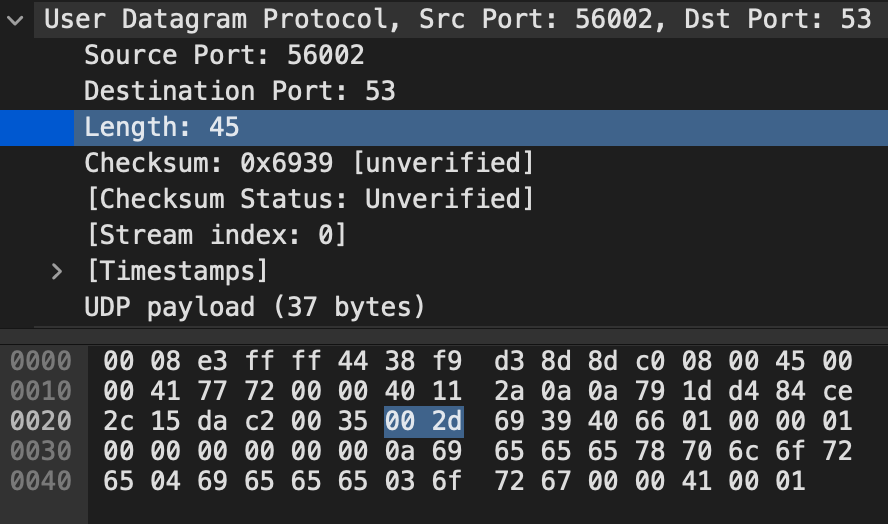
\includegraphics[width=\textwidth]{subfiles/images/ECSE_308_Lab_5_1_SUPA_PAGE7_22_Image61.png}
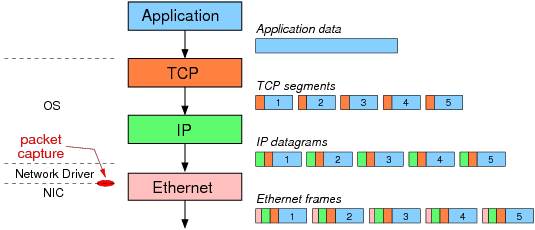
\includegraphics[width=\textwidth]{subfiles/images/L5_Manual/L5N2_ DNS & HTTP_PAGE24_13_Image153.png
}
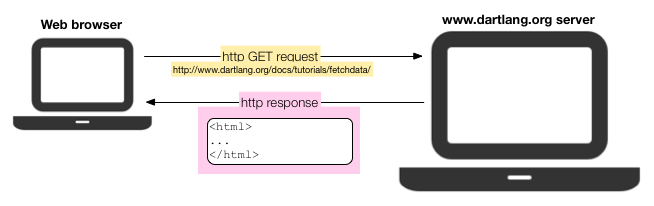
\includegraphics[width=\textwidth]{subfiles/images/L5_Manual/L5N2_ DNS & HTTP_PAGE21_12_Image137.png}
\subfile{./Folland/Theorem4_14.tex}
\subfile{./Folland/Theorem4_15.tex}
\subfile{./Folland/Theorem4_16.tex}
\end{proof}

\end{document}